
	\chapter{RESULTS \& DISCUSSION}
	\label{chap:results}
		In the proposed systems the inclusion of `EVs' gives rise to an increase in power loss this and the pros of the charging scheme could be verified via the tables given below.
	\section{Tabulations}
	The datas given below are about the Most Economic Time interval to Charge the Vehicle, charging Patterns and Voltage magnitude graphs for different scenarios.
		\subsection{Economic Charging}
		
			Three cases are taken in this study which are namely:
				Case 1(00:00): Case 1 depicts that the vehicles has Started on a hourly basis i.e. the 1 hour block.
				Case 2(00:20) : Case 2 depicts that the vehicle has Started from the 20th min of an hour i.e. 20mins block.
				Case 3(00:40): Case 3 depicts that the vehicles has Started from the 40th minute of an hour i.e. 40th minute block
			
			\begin{table}[!h]
				\caption{Most Economic Time interval to Charge the Vehicle}
				\centering
			\begin{tabular}{|l|l|l|l|}
				\hline
				\textbf{VEHICLE TYPE}           & \textbf{CASE}         & \textbf{BEST PRICE} & \textbf{HOUR} \\ \hline
				\multirow{3}{*}{\textbf{CAR}}   & \textbf{Case 1 - (00:00)} & - \$1.71            & 12:00         \\ \cline{2-4} 
				& \textbf{Case 2 - (00:20)} & - \$2.09            & 01:20         \\ \cline{2-4} 
				& \textbf{Case 3 - (00:40)} & - \$1.58            & 01:40         \\ \hline
				\multirow{3}{*}{\textbf{BUS}}   & \textbf{Case 1 - (00:00)} & - \$0.47            & 12:00         \\ \cline{2-4} 
				& \textbf{Case 2 - (00:20)} & - \$1.25            & 20:20         \\ \cline{2-4} 
				& \textbf{Case 3 - (00:40)} & - \$0.69            & 11:40         \\ \hline
				\multirow{3}{*}{\textbf{TRUCK}} & \textbf{Case 1 - (00:00)} & - \$2.57            & 05:00         \\ \cline{2-4} 
				& \textbf{Case 2 - (00:20)} & -\$1.00             & 04:20         \\ \cline{2-4} 
				& \textbf{Case 3 - (00:40)} & - \$2.11            & 04:40         \\ \hline
			\end{tabular}
		\end{table}
		
		Using the above table we can identify the best economic time to charge and how much will it cost at the most economic time.

	\subsection{Maximum EV Load}
	
		In the provided table \ref{table:whichbus} the power loss is calculated in such a way that the time blocks having the maximum load  is considered and then load flow analysis is performed on 2nd bus(best case)and 18th bus( worst case) of 33 bus system to find the variation of load with and without EV .
		
			\begin{table}[!h]
			\centering
			\caption{Hour at which the EV Load is maximum }
			\begin{tabular}{|ll|ll|ll|ll|}
				\hline
				\multicolumn{2}{|l|}{\textbf{SCENARIO}} & \multicolumn{2}{l|}{\textbf{HOURLY}} & \multicolumn{2}{l|}{\textbf{20MINS}} & \multicolumn{2}{l|}{\textbf{40 MINS}} \\ \hline
				\multicolumn{2}{|l|}{\textbf{SCENARIO-1}}        & \multicolumn{2}{l|}{$ 13^{th} $}            & \multicolumn{2}{l|}{$ 6^{th} $}             & \multicolumn{2}{l|}{$ 13^{th} $}             \\ \hline
				\multicolumn{2}{|l|}{\textbf{SCENARIO-2}}        & \multicolumn{2}{l|}{$ 19^{th} $}           & \multicolumn{2}{l|}{$ 6^{th} $}             & \multicolumn{2}{l|}{$ 19^{th} $}             \\ \hline
			\end{tabular}
			\label{table:whichbus}
		\end{table}
	

	
	\subsection{Power Loss}
	
	
		\begin{table}[!h]
			\centering
			\caption{Power Loss when EV is connected in a 33 bus system}
			\begin{tabular}{|c|c|cc|cc|cc|}
				\hline
				\multirow{2}{*}{\textbf{Scenario}}                            & \multirow{2}{*}{\textbf{\begin{tabular}[c]{@{}c@{}}Base\\ Case\\ Power\\ Loss\end{tabular}}} & \multicolumn{2}{c|}{\textbf{Case 1}}                                                                                                                                                                          & \multicolumn{2}{c|}{\textbf{Case 2}}                                                                                                                                                                          & \multicolumn{2}{c|}{\textbf{Case 3}}                                                                                                                                                                          \\ \cline{3-8} 
				&                                                                                              & \multicolumn{1}{c|}{\textbf{\begin{tabular}[c]{@{}c@{}}Power \\ Loss\\ when EV\\ in Bus 2\\ (kW)\end{tabular}}} & \textbf{\begin{tabular}[c]{@{}c@{}}Power \\ Loss\\ when EV\\ in Bus 18\\ (kW)\end{tabular}} & \multicolumn{1}{c|}{\textbf{\begin{tabular}[c]{@{}c@{}}Power \\ Loss\\ when EV\\ in Bus 2\\ (kW)\end{tabular}}} & \textbf{\begin{tabular}[c]{@{}c@{}}Power \\ Loss\\ when EV\\ in Bus 18\\ (kW)\end{tabular}} & \multicolumn{1}{c|}{\textbf{\begin{tabular}[c]{@{}c@{}}Power\\  Loss\\ when EV\\ in Bus 2\\ (kW)\end{tabular}}} & \textbf{\begin{tabular}[c]{@{}c@{}}Power \\ Loss\\ when EV\\ in Bus 18\\ (kW)\end{tabular}} \\ \hline
				\textbf{\begin{tabular}[c]{@{}c@{}}Scenario\\ 1\end{tabular}} & \multirow{2}{*}{202.691}                                                                     & \multicolumn{1}{c|}{204.104}                                                                                    & 253.746                                                                                     & \multicolumn{1}{c|}{65.773}                                                                                     & 78.460                                                                                      & \multicolumn{1}{c|}{204.104}                                                                                    & 253.746                                                                                     \\ \cline{1-1} \cline{3-8} 
				\textbf{\begin{tabular}[c]{@{}c@{}}Scenario\\ 2\end{tabular}} &                                                                                              & \multicolumn{1}{c|}{189.833}                                                                                    & 236.912                                                                                     & \multicolumn{1}{c|}{178.967}                                                                                    & 222.468                                                                                     & \multicolumn{1}{c|}{189.833}                                                                                    & 236.912                                                                                     \\ \hline
			\end{tabular}
						\label{table:powerloss}
		\end{table}





		
		
		
		
		
		
		
	\section{Charging Patterns}
		These plots depict the charging and discharging pattern for the classified vehicles. 216 vehicles are taken into consideration for each vehicle type and the charging pattern is identified.
		
		\noindent A strategic pattern is established to maintain the stability of the grid by comparing the vehicle capacity to the Real time price for each hour. When the price is low, the vehicle is put to charge and when the price is high,the vehicle is put to discharge in comparision with the peak demand. By this way the overall cost is drastically reduced , leading to profit for the user and at the same time the overall load in the grid decreases making the load demand cure flatter.
		
		\begin{figure}[!h]
		\centering
		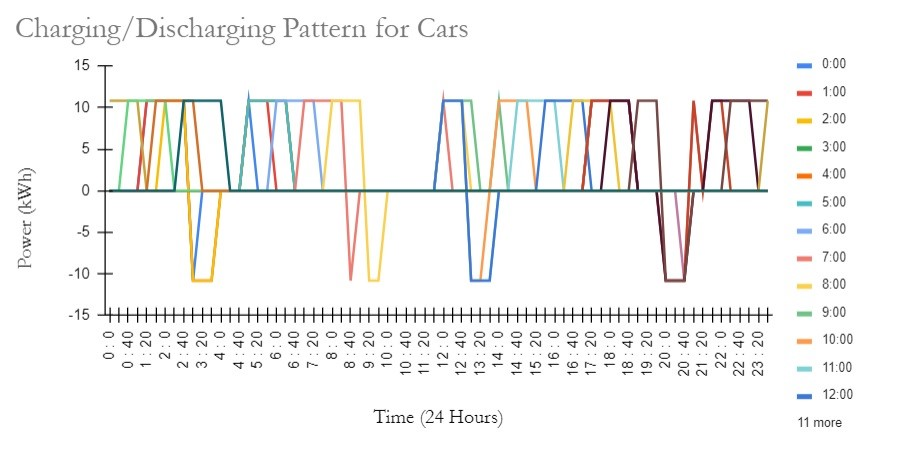
\includegraphics[width=0.7\linewidth]{Figures/cp_case1}
		\caption{Charging/Discharging pattern for Cars}
		\label{fig:cpcase1}
		\end{figure}
	
		\begin{figure}[!h]
		\centering
		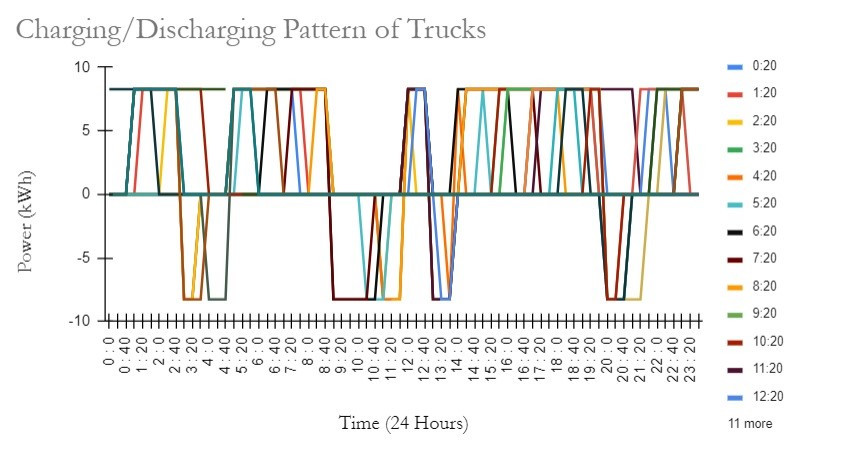
\includegraphics[width=0.7\linewidth]{Figures/cp_case2}
		\caption{Charging/Discharging pattern for Trucks}
		\label{fig:cpcase2}
		\end{figure}
	
		\begin{figure}[!h]
			\centering
			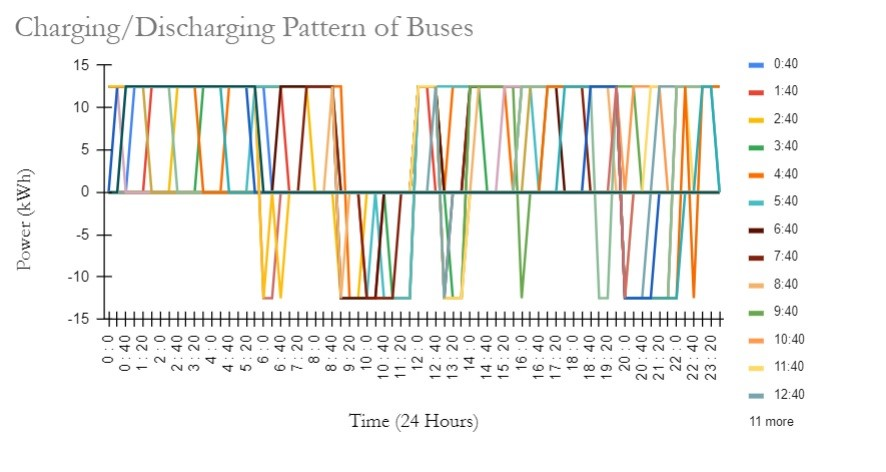
\includegraphics[width=0.7\linewidth]{Figures/cp_case3}
			\caption{Charging/Discharging pattern for Buses}
			\label{fig:cpcase3}
		\end{figure}


			
			
			
			
			
			
			
	\section{Voltage Magnitude Graphs for Different Scenarios}
	
	The voltage magnitude of the base case and each time block for  all the cases are computed. Load flow analysis is done on Bus number 2 and Bus number 18 as these are considered to be the best case and worst case buses to calculate the voltage magnitude as referred from \cite{33bus}. From the results it is evident that the loss difference in the grid without EVs connected to the grid(base case) and with EVs connected to the grid on bus number 2 are comparatively lesser. The same loss difference is higher when the EVs connected in 18th bus is high. Looking into voltage magnitude the value of voltage magnitude in base case and EVs connected to the grid on 2nd bus are equal. Whereas in 18th bus it is clear that voltage magnitude when compared to base case is high.
	
	\noindent Here figures (\ref{fig:LFa}), (\ref{fig:LFb}) and  (\ref{fig:LFc}) shows the voltage magnitude plot when the EVs are connected to bus 2 and bus 18 during various cases.

	\noindent and figures (\ref{fig:LF2a}), (\ref{fig:LF2b}) and  (\ref{fig:LF2c}) shows the voltage magnitude plot when the EVs are connected to bus 2 and bus 18 during various cases.
	
	 \begin{figure}[!h]
		\begin{subfigure}{.5\textwidth}
			\centering
			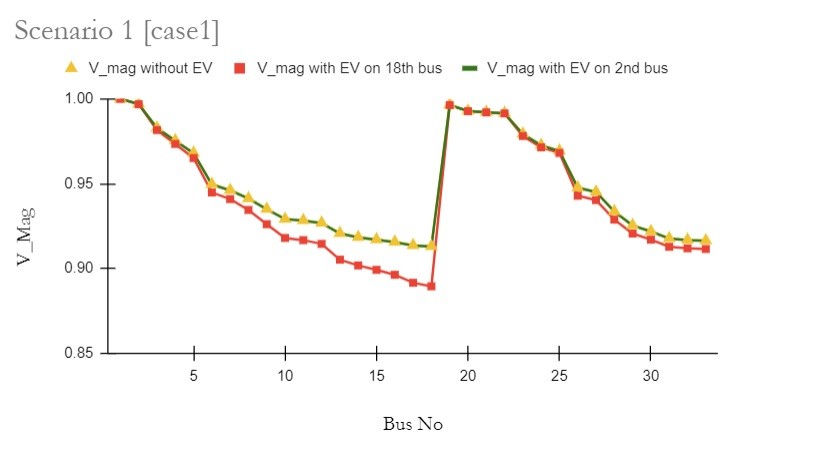
\includegraphics[width=.97\linewidth,height= 4.95cm]{./Figures/sc1_case1}  
			\caption{Case I}
			\label{fig:LFa}
		\end{subfigure}
		\begin{subfigure}{.5\textwidth}
			\centering
			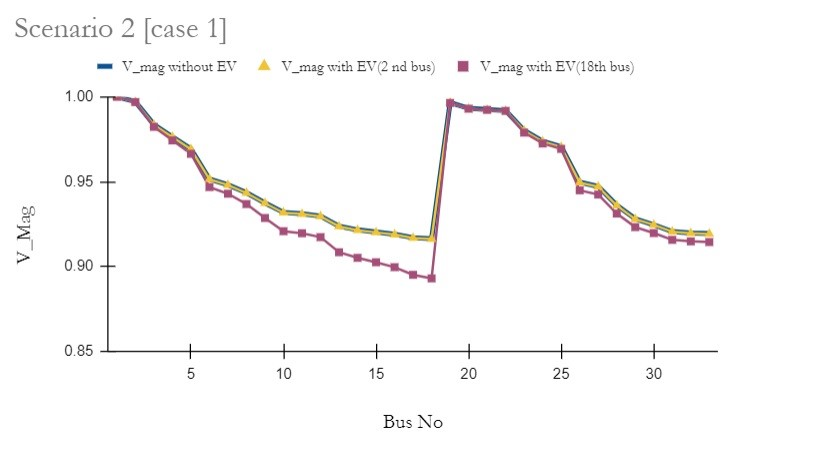
\includegraphics[width=.97\linewidth,height= 4.95cm]{./Figures/sc2_case1}  
			\caption{Case I}
			\label{fig:LF2a}
		\end{subfigure}
		\begin{subfigure}{.5\textwidth}
			\centering
			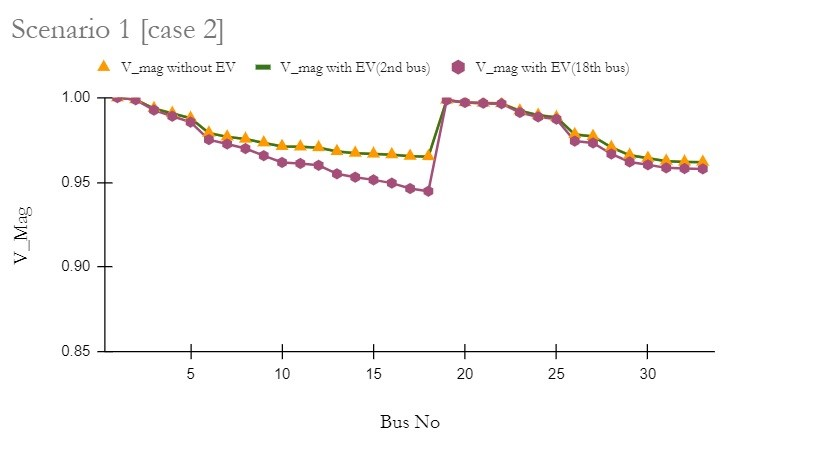
\includegraphics[width=.97\linewidth,height= 4.95cm]{./Figures/sc1_case2}
			\caption{Case II}
			\label{fig:LFb}
		\end{subfigure}
		\begin{subfigure}{.5\textwidth}
			\centering
			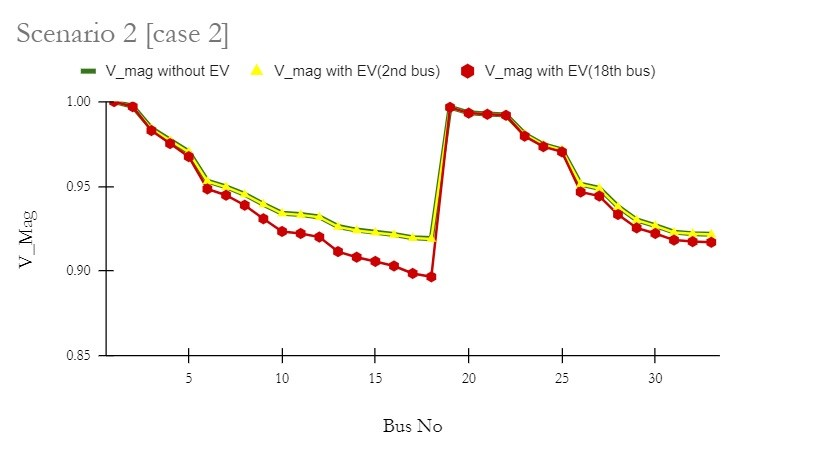
\includegraphics[width=.97\linewidth,height= 4.95cm]{./Figures/sc2_case2}
			\caption{Case II}
			\label{fig:LF2b}
		\end{subfigure}
		\begin{subfigure}{.5\textwidth}
			\centering
			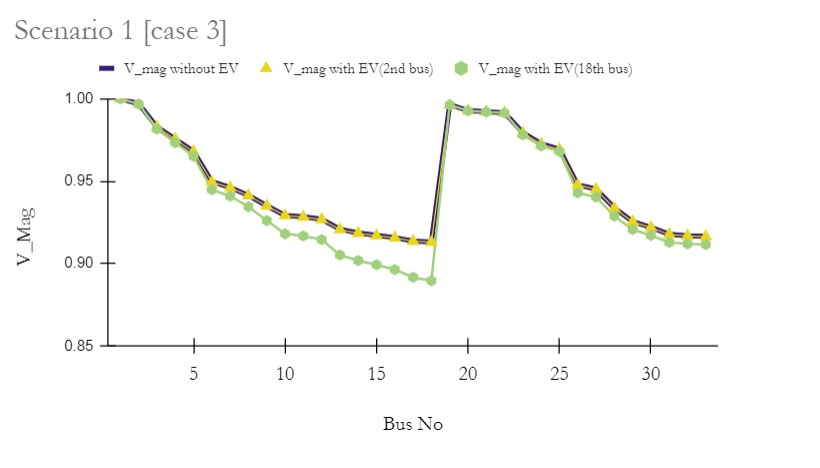
\includegraphics[width=.97\linewidth,height= 4.95cm]{./Figures/sc1_case3}
			\caption{Case III}
			\label{fig:LFc}
		\end{subfigure}
		\begin{subfigure}{.5\textwidth}
			\centering
			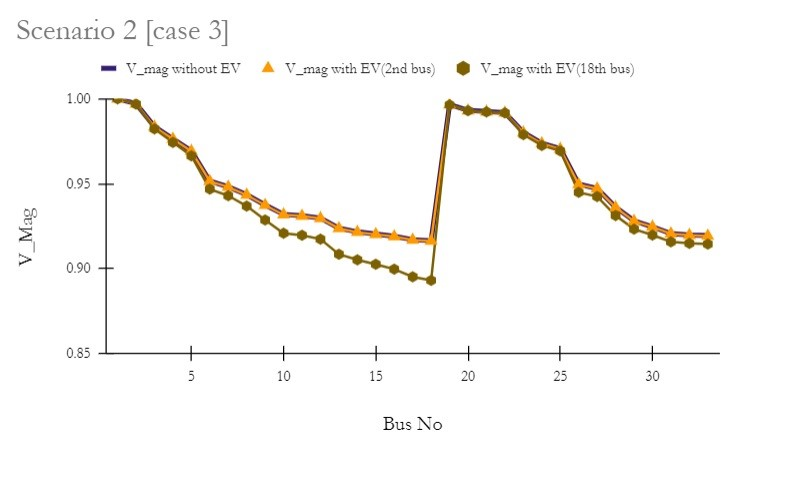
\includegraphics[width=.97\linewidth,height= 4.95cm]{./Figures/sc2_case3}
			\caption{Case III}
			\label{fig:LF2c}
		\end{subfigure}
		\caption{ Voltage magnitude variation for different scenarios }
		\label{fig:loadprofile-scenario1}
	\end{figure} 
	
	


		
	
	
	